\documentclass[xcolor=dvipsnames]{beamer}
\usetheme{CambridgeUS}
\usepackage[labelformat=simple,
labelsep=period,
font={footnotesize},     %scriptsize, footnotesize, small, normalsize
labelfont=bf,
width=0.9\textwidth,
justification=justified,
singlelinecheck=false
]{caption}
\usepackage[utf8]{inputenc}
\usepackage[spanish, es-tabla]{babel}
\usepackage{amsmath}
\usepackage{subfigure}
\usepackage{amsfonts}
\usepackage{amssymb}
\usepackage{qtree}
\usepackage{tikz}
\usetikzlibrary{calc}
\usepackage{pgfplots,pgfplotstable}
\usepgfplotslibrary{statistics}
\usepackage[T1]{fontenc}
\usepackage{bera}
\usepackage{multirow}
\usepackage{pstricks-add}
\usepackage[capposition=top]{floatrow}
\usepackage{graphicx}
 \usepackage{ragged2e}
 \usepackage{float}
 \usepackage[labelformat=simple,
 labelsep=period,
 font={footnotesize},     %scriptsize, footnotesize, small, normalsize
 labelfont=bf,
 width=0.9\textwidth,
 justification=justified,
 singlelinecheck=false
 ]{caption}
 \usepackage[justification=centering]{caption}
\setbeamersize{text margin left=5pt,text margin right=25pt}
\captionsetup[figure]{labelfont={color=Brown}}
\captionsetup[table]{labelfont={color=Brown}}

\pgfplotsset{compat=1.7}

%%%%%%%%%%%%%%%%%%%%%%%%%%%%%%%%%%%%%%%%%%%%%%%%%%%%%%%%
%%% PAra el diagrama de la diapostiva 10
\usepackage{smartdiagram}
\usetikzlibrary{shapes.geometric} % required in the preamble
\smartdiagramset{
	module minimum width=3cm,
	module minimum height=1cm,
	text width=4.5cm,
	circular distance=3cm,
}
%%%%%%%%%%%%%%%%%%%%%%%%%%%%%%%%%%%%%%%%%%%%%%%%%%%%%%%%%%%
\def\angle{0}
\def\radius{2}
\def\cyclelist{{"orange","blue","red","green"}}
\newcount\cyclecount \cyclecount=-1
\newcount\ind \ind=-1	


\newcounter{saveenumi}
\newcommand{\seti}{\setcounter{saveenumi}{\value{enumi}}}
\newcommand{\conti}{\setcounter{enumi}{\value{saveenumi}}}

\resetcounteronoverlays{saveenumi}
	\tikzset{mynode/.style={inner sep=2pt,fill,outer sep=0,circle}}
	
\author[Carlos Cardona]{Carlos Cardona}
\title{Análisis Cuantitativo I}
\subtitle{Probabilidad}
\institute[URosario]{Universidad del Rosario}
\date{19 de agosto de 2016}
\begin{document}
	\pgfmathdeclarefunction{gauss}{2}{\pgfmathparse{1/(#2*sqrt(2*pi))*exp(-((x-#1)^2)/(2*#2^2))}%
	}
\maketitle

%%%%%%%%%%%%%%%%%%%%%%%%%%%%%%%%%%%%%%%%%%%%%%%%%%%%%%
\section{Percentiles}
\begin{frame}{Distribución Porcentual Acumulada}
\begin{itemize}
\justifying
\item Además de la proporción y el porcentaje, una tabla de distribución de frecuencia puede incluir información de la frecuencia porcentual acumulada.
\begin{center}
\begin{table}[H]
\begin{tabular}{ccccc} \hline
Edad(X) & $f$ & Proporción & Porcentaje (\%) & \% Acumulado \\ \hline
18 &1& $\frac{1}{10}=0.1$ & 10 & 10 \\
19 &3 & $\frac{3}{10}=0.3$ &30 &40 \\
20 &2 & $\frac{2}{10}=0.2$ &20 &60 \\
21 &1 & $\frac{1}{10}=0.1$ &10 &70 \\
22 &3 & $\frac{3}{10}=0.3$ &30 &100 \\ \hline
\end{tabular}
\end{table}
\end{center}
\item Esta frecuencia porcentual acumulada me permite dividir la distribución según cuántas observaciones están por debajo de un valor.
\end{itemize}
\end{frame}

\begin{frame}{Percentil}
\begin{itemize}
\justifying
\item Utilizar percentiles es la manera más común, dividiendo una distribución en 100.
\item Describe el porcentaje de casos que son menores o iguales a un valor específico.
\item Por ejemplo, en la tabla anterior, 21 años es el percentil 70. 
$$p(edad\leq20)=\dfrac{6}{10}=0.6*100=60\%$$
\item Por tanto, 20 es el percentil 60.
\item ¿Cuál es el percentil 50?
\end{itemize}
\end{frame}

\begin{frame}{Cuartil y Decil}
\begin{itemize}
\justifying
\item Los cuartiles y deciles dividen la distribución en 4 y 10 partes, respectivamente. 
\item Con respecto a los cuartiles:
\begin{center}
\begin{table}[H]
\begin{tabular}{cc} \hline
Cuartil & Percentil \\ \hline
$Q_1$ & 25 \\
$Q_2$ & 50 \\
$Q_3$ & 75 \\
$Q_4$ & 100 \\ \hline
\end{tabular}
\end{table}
\end{center}
\item Por otro lado, el primer decil es el percentil 10, el segundo es el percentil 20,..., etc.
\end{itemize}
\end{frame}
%%%%%%%%%%%%%%%%%%%%%%%%%%%%%%%%%%%%%%%%%%%%%%%%%%%%%%%
\section{Probabilidad}

\begin{frame}{Probabilidad}
\begin{itemize}
\justifying
\item Una investigación inicia con una pregunta general sobre una población entera, pero se realiza usando una muestra.
\item En esta situación, el rol de la estadística inferencial es utilizar la muestra como base para generalizar los resultados a la población.
\item Para lograr este objetivo, los procedimiento inferenciales están construidos sobre el concepto de probabilidad.
\item Específicamente, la relación entre población y muestra usualmente se define en términos de probabilidad.
\end{itemize}
\end{frame}

\begin{frame}
\begin{itemize}
\justifying
\item Supongamos, por ejemplo, que seleccionamos una canica de un frasco que contiene 50 canicas negras y 50 canicas blancas.
\item Aunque no podemos garantizar el color, sabemos que existe una probabilidad de 50-50 de obtener cualquiera de ambos colores.
\item Consideremos ahora otro frasco (población) que tiene 90 canicas negras y 10 blancas.
\item Nuevamente no podemos garantizar el resultado de la muestra, pero es probable que sea de color negro.
\item La probabilidad es una conexión entre población y muestra, la cual es base para la estadística inferencial que veremos más adelante.
\end{itemize}
\end{frame}

\begin{frame}{¿Qué es Probabilidad?}
\begin{block}{Probabilidad}
	\justifying
Una probabilidad es una estimación de con qué frecuencia es posible que ocurra un evento de interés particular entre un gran número de ensayos.
\end{block}
\begin{itemize}
\justifying
\item Una probabilidad se define como la siguiente proporción
: 
$$P=\dfrac{\#\, resultados\, deseados}{\#\, resultados\, posibles}$$
\item Por ejemplo, al tirar un dado la probabilidad de obtener un 2 luego de lanzar un dado es:
$$P(2)=\dfrac{1}{6}=0.166=16.66\%$$
\end{itemize}
\end{frame}

\begin{frame}{Reglas básicas de la Probabilidad}
\begin{enumerate}
\justifying
\item Las probabilidades siempre están entre 0 y 1.
\begin{itemize}
	
\item Una probabilidad igual a 0 indica que el evento nunca va a ocurrir. 
\item Por otro lado, si es igual 1 indica que con toda seguridad el evento tendrá lugar.
\end{itemize}
\item $\sum{P}=1$
\item La probabilidad que un evento {\bf no ocurra} es igual a 1 menos la probabilidad que el evento ocurra.
\begin{itemize}
\item Al tirar un dado:
$$P(\sim2)=1-P(2)=1-\dfrac{1}{6}=\dfrac{5}{6}$$
\end{itemize}
 \seti
\end{enumerate}
\end{frame}
\begin{frame}
\begin{enumerate}
	\justifying
\conti
\item Si A y B son eventos alternativos (no se superponen), entonces $P(A$ $o$ $B)=P(A)+P(B)$
\begin{itemize}
\item Siguiendo con el ejemplo del dado:
$$P(2\, o\,  3)=P(2)+P(3)=\dfrac{1}{6}+\dfrac{1}{6}=\dfrac{2}{6}=\dfrac{1}{3}$$
\end{itemize}
\item Si A y B son eventos que se superponen (ocurrencia conjunta), entonces $P(A$ $o$ $B)=P(A)+P(B)-P(A$ $y$ $B)$
\begin{itemize}
\item ¿Cuál sería la probabilidad de sacar un número par o un 6?
$$P(Par\, o\,  6)=P(Par)+P(6)=\dfrac{3}{6}+\dfrac{1}{6}=\dfrac{4}{6}=\dfrac{2}{3} \quad Incorrecto $$
$$P(Par\, o\,  6)=P(Par)+P(6)-P(Par\, y\,  6)=\dfrac{3}{6}+\dfrac{1}{6}-\dfrac{1}{6}=\dfrac{3}{6}=\dfrac{1}{2} \quad Correcto $$
\end{itemize}
\seti
\end{enumerate}

\end{frame}

\begin{frame}
\begin{enumerate}
	\justifying
	\conti
\item Si A y B son {\bf independientes}, entonces $P(A\, y\, B)=P(A)*P(B)$
\begin{itemize}
\item ¿Cuál es la probabilidad de sacar 2 luego de tirar el dados dos veces?
$$P(2\, luego\, 2)=P(2)*P(2)=\dfrac{1}{6}*\dfrac{1}{6}=\dfrac{1}{36}$$
\item Es importante tener en cuenta si existe reemplazo o no.
\item Por ejemplo, si un recipiente tiene 4 pelotas amarrilas y 2 azules. ¿Cuál es la probabilidad de sacar una amarilla y luego una azul sin reemplazo?
$$P(Amarilla\, luego\, Azul)=P(Amarilla)*P(Azul)=\dfrac{4}{6}*\dfrac{2}{5}=\dfrac{8}{30}=\dfrac{4}{15}$$
\end{itemize}
\end{enumerate}
\end{frame}
%%%%%%%%%%%%%%%%%%%%%%%%%%%%%%%%%%%%%%%%%%%%%%%%
\section{Probabilidad y la Distribución Normal}
\begin{frame}{Probabilidad y la Distribución Normal}
	\begin{center}
		\scalebox{0.9}{
			\begin{tikzpicture}
			\begin{axis}[no markers, domain=0:10, samples=100,
			axis lines*=left, xlabel=Desviaciones estándar, ylabel=Frecuencia,,
			height=6cm, width=10cm,
			xtick={-3, -2, -1, 0, 1, 2, 3}, ytick=\empty,
			enlargelimits=false, clip=false, axis on top,
			grid = major]
			\addplot [fill=cyan!20, draw=none, domain=-3:3] {gauss(0,1)} \closedcycle;
			\addplot [fill=orange!20, draw=none, domain=-3:-2] {gauss(0,1)} \closedcycle;
			\addplot [fill=orange!20, draw=none, domain=2:3] {gauss(0,1)} \closedcycle;
			\addplot [fill=blue!20, draw=none, domain=-2:-1] {gauss(0,1)} \closedcycle;
			\addplot [fill=blue!20, draw=none, domain=1:2] {gauss(0,1)} \closedcycle;
			\addplot[] coordinates {(-1,0.4) (1,0.4)};
			\addplot[] coordinates {(-2,0.3) (2,0.3)};
			\addplot[] coordinates {(-3,0.2) (3,0.2)};
			\node[coordinate, pin={68.2\%}] at (axis cs: 0, 0.4){};
			\node[coordinate, pin={95\%}] at (axis cs: 0, 0.3){};
			\node[coordinate, pin={99.7\%}] at (axis cs: 0, 0.2){};
			\node[coordinate, pin={34.1\%}] at (axis cs: -0.5, 0){};
			\node[coordinate, pin={34.1\%}] at (axis cs: 0.5, 0){};
			\node[coordinate, pin={13.6\%}] at (axis cs: 1.5, 0){};
			\node[coordinate, pin={13.6\%}] at (axis cs: -1.5, 0){};
			\node[coordinate, pin={2.1\%}] at (axis cs: 2.5, 0){};
			\node[coordinate, pin={2.1\%}] at (axis cs: -2.5, 0){};
			\end{axis}
			\end{tikzpicture}}
	\end{center}
\end{frame}

\begin{frame}{Tabla de la Distribución Normal}
	\begin{figure}[H]  
		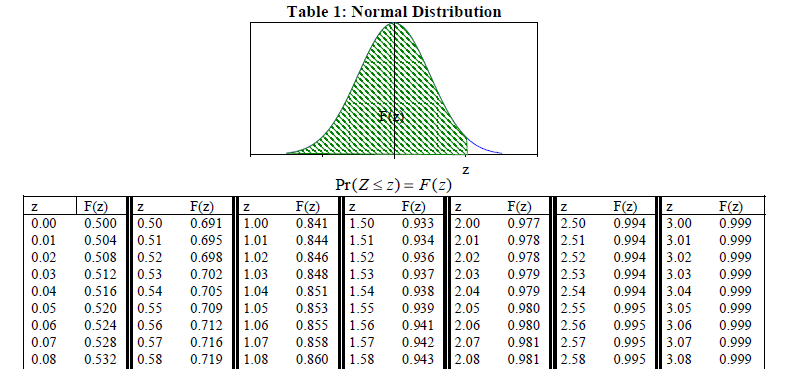
\includegraphics[width = 1\textwidth]{./cap3}
	\end{figure}
\end{frame}

\begin{frame}{Algunos ejemplos}
	\begin{figure}[H]
		\centering  
		\caption{ } 
		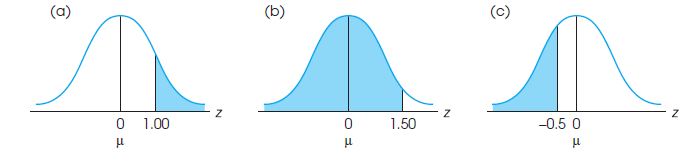
\includegraphics[width = 1\textwidth]{./cap1}
	\end{figure}
\end{frame}

\begin{frame}{Algunos ejemplos}
	\begin{figure}[H]
		\centering  
		\caption{ } 
		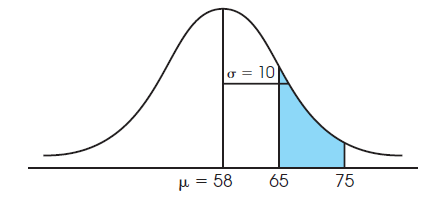
\includegraphics[width = 1\textwidth]{./cap2}
	\end{figure}
\end{frame}

\begin{frame}{Algunos ejemplos}
	\begin{figure}[H]
		\centering  
		\caption{ } 
		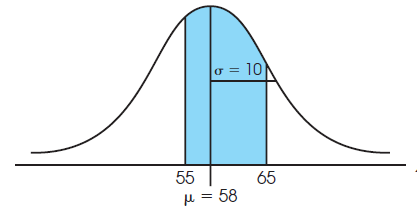
\includegraphics[width = 0.9\textwidth]{./cap4}
	\end{figure}
\end{frame}

\begin{frame}
	\begin{center}
		\scalebox{1}{
			\begin{tikzpicture}
			% define normal distribution function 'normaltwo'
			\def\normaltwo{\x,{4*1/exp(((\x-3)^2)/2)}}
			
			% input y parameter
			\def\x{1.9}
			\def\y{4.05}
			\def\z{3.01}
			% this line calculates f(y)
			\def\fx{4*1/exp(((\x-3)^2)/2)}
			\def\fy{4*1/exp(((\y-3)^2)/2)}
			\def\fz{4*1/exp(((\z-3)^2)/2)}
			% Shade orange area underneath curve.
			\fill [fill=green!60] (\x,0) -- plot[domain=\x:\y] (\normaltwo) -- ({\y},0) -- cycle;	
			% Draw and label normal distribution function
			\draw[color=blue,domain=0:6] plot (\normaltwo) node[right] {};
			
			% Add dashed line dropping down from normal.
			\draw[dashed] ({\x},{\fx}) -- ({\x},0) node[below] {$-1$};
			\draw[dashed] ({\y},{\fy}) -- ({\y},0) node[below] {$0.9$};
			\draw[dashed] ({\z},{\fz}) -- ({\z},0) node[below] {$0$};
			% Optional: Add axis labels
			\draw (-.2,2.5) node[left] {$f_x$};
			\draw (3,-.5) node[below] {$x$};
			
			% Optional: Add axes
			\draw[->] (0,0) -- (6.2,0) node[right] {};
			\draw[->] (0,0) -- (0,5) node[above] {};
			
			\end{tikzpicture}
		}
	\end{center}
\end{frame}

\begin{frame}\frametitle{test}
	\begin{columns}
		\begin{column}{.49\textwidth}
			\centering
			\only<1>{The plot of $\exp x$}\\[1ex]
			\scalebox{0.8}{
				\begin{tikzpicture}
				% define normal distribution function 'normaltwo'
				\def\normaltwo{\x,{4*1/exp(((\x-3)^2)/2)}}
				
				% input y parameter
				\def\y{4.4}
				\def\z{3.01}
				% this line calculates f(y)
				\def\fy{4*1/exp(((\y-3)^2)/2)}
				\def\fz{4*1/exp(((\z-3)^2)/2)}
				% Shade orange area underneath curve.
				\fill [fill=orange!60] (2.6,0) -- plot[domain=0:4.4] (\normaltwo) -- ({\y},0) -- cycle;
				
				% Draw and label normal distribution function
				\draw[color=blue,domain=0:6] plot (\normaltwo) node[right] {};
				
				% Add dashed line dropping down from normal.
				\draw[dashed] ({\y},{\fy}) -- ({\y},0) node[below] {$1$};
				\draw[dashed] ({\z},{\fz}) -- ({\z},0) node[below] {$0$};
				% Optional: Add axis labels
				\draw (-.2,2.5) node[left] {$f_x$};
				\draw (3,-.5) node[below] {$x$};
				
				% Optional: Add axes
				\draw[->] (0,0) -- (6.2,0) node[right] {};
				\draw[->] (0,0) -- (0,5) node[above] {};
				
				\end{tikzpicture}}
		\end{column}
		
		\begin{column}{.49\textwidth}
			\centering
			\only<1>{The plot of $\sin x$}\\[1ex]
			\scalebox{0.8}{
				\begin{tikzpicture}
				% define normal distribution function 'normaltwo'
				\def\normaltwo{\x,{4*1/exp(((\x-3)^2)/2)}}
				
				% input y parameter
				\def\x{1.6}
				\def\y{6}
				\def\z{3.01}
				% this line calculates f(y)
				\def\fx{4*1/exp(((\x-3)^2)/2)}
				\def\fy{4*1/exp(((\y-3)^2)/2)}
				\def\fz{4*1/exp(((\z-3)^2)/2)}
				% Shade orange area underneath curve.
				\fill [fill=green!60] (\x,0) -- plot[domain=\x:\y] (\normaltwo) -- ({\y},0) -- cycle;	
				% Draw and label normal distribution function
				\draw[color=blue,domain=0:6] plot (\normaltwo) node[right] {};
				
				% Add dashed line dropping down from normal.
				\draw[dashed] ({\x},{\fx}) -- ({\x},0) node[below] {$-1$};
				\draw[dashed] ({\y},{\fy}) -- ({\y},0) node[below] {};
				\draw[dashed] ({\z},{\fz}) -- ({\z},0) node[below] {$0$};
				% Optional: Add axis labels
				\draw (-.2,2.5) node[left] {$f_x$};
				\draw (3,-.5) node[below] {$x$};
				
				% Optional: Add axes
				\draw[->] (0,0) -- (6.2,0) node[right] {};
				\draw[->] (0,0) -- (0,5) node[above] {};
				
				\end{tikzpicture}}
			
		\end{column}
	\end{columns}
\end{frame}
\end{document}